

\section{Prueba 3}

\subsection{Red de inferencia}
\par Esta red de inferencia se debe interpretar de izquierda a derecha.
Los rectángulos azules son las reglas, los grises que están ligados por la izquierda 
de ellas son sus antecedentes, si estos antecedentes convergen en un cuadrado 
quiere decir que es la conjunción de esos literales, en caso contrario son disyunciones
o simplemente un literal. Los rectángulos grises unidos a las reglas por la derecha
son sus consecuentes respectivamente. Además, incluyo los factores de certeza propocionados por
la Base de hechos y la Base de Conocimiento iniciales.

\begin{center}
	\tikzstyle{regla}= [rectangle,draw,black,fill=blue!15]
	\tikzstyle{hecho}= [rectangle,draw,black,fill=black!15]
	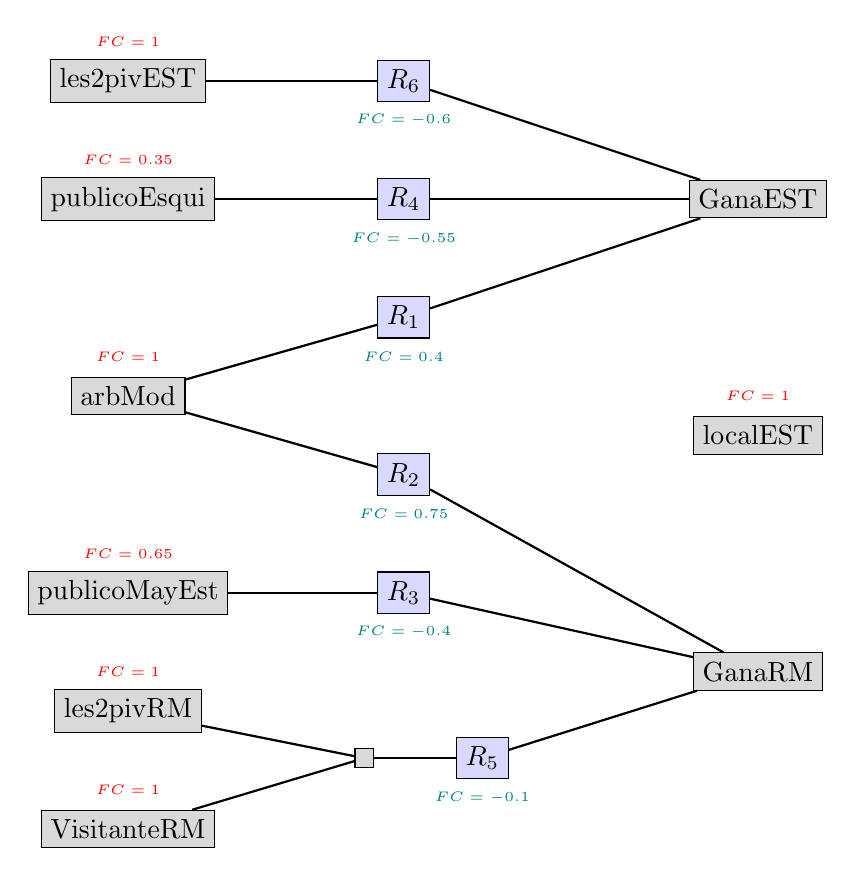
\begin{tikzpicture}
			
		\node (a) at (8,6.5) [hecho] {localEST};
		\node at (8,7) {\color{red}{\tiny{$FC=1$}}};

		\node (b) at (0,1.5) [hecho] {VisitanteRM};
		\node at (0,2) {\color{red}{\tiny{$FC=1$}}};

		\node (c) at (0,7) [hecho] {arbMod};
		\node at (0,7.5) {\color{red}{\tiny{$FC=1$}}};

		\node (d) at (0,4.5)[hecho] {publicoMayEst};
		\node at (0,5) {\color{red}{\tiny{$FC=0.65$}}};

		\node (e) at (0,9.5)[hecho] {publicoEsqui};
		\node at (0,10) {\color{red}{\tiny{$FC=0.35$}}};

		\node (f) at (0,11)[hecho] {les2pivEST};
		\node at (0,11.5) {\color{red}{\tiny{$FC=1$}}};

		\node (g) at (0,3)[hecho] {les2pivRM};
		\node at (0,3.5) {\color{red}{\tiny{$FC=1$}}};

		\node (h) at (8,9.5)[hecho] {GanaEST};

		\node (i) at (8,3.5)[hecho] {GanaRM};

		\node (g/b) at (3,2.4)[hecho] {};

		\node (r1) at (3.5,8) [regla] {$R_{1}$};
		\node at (3.5,7.5) {\color{teal}{\tiny{$FC=0.4$}}};
		\node (r2) at (3.5,6) [regla] {$R_{2}$};
		\node at (3.5,5.5) {\color{teal}{\tiny{$FC=0.75$}}};
		\node (r3) at (3.5,4.5) [regla] {$R_{3}$};
		\node at (3.5,4) {\color{teal}{\tiny{$FC=-0.4$}}};
		\node (r4) at (3.5,9.5) [regla] {$R_{4}$};
		\node at (3.5,9) {\color{teal}{\tiny{$FC=-0.55$}}};
		\node (r5) at (4.5,2.4) [regla] {$R_{5}$};
		\node at (4.5,1.9) {\color{teal}{\tiny{$FC=-0.1$}}};
		\node (r6) at (3.5,11) [regla] {$R_{6}$};
		\node at (3.5,10.5) {\color{teal}{\tiny{$FC=-0.6$}}};

		\path[black,thick] (f) edge[] node {} (r6);
		\path[black,thick] (r6) edge[] node {} (h);
		\path[black,thick] (e) edge[] node {} (r4);
		\path[black,thick] (r4) edge[] node {} (h);
		\path[black,thick] (c) edge[] node {} (r1);
		\path[black,thick] (r1) edge[] node {} (h);

		\path[black,thick] (c) edge[] node {} (r2);
		\path[black,thick] (r2) edge[] node {} (i);
		\path[black,thick] (d) edge[] node {} (r3);
		\path[black,thick] (r3) edge[] node {} (i);
		\path[black,thick] (g) edge[] node {} (g/b);
		\path[black,thick] (b) edge[] node {} (g/b);
		\path[black,thick] (g/b) edge[] node {} (r5);
		\path[black,thick] (r5) edge[] node {} (i);

	\end{tikzpicture}
\end{center}


\subsection{Proceso de inferencia con Objetivo \texttt{ganaEst}}
\begin{listing}[language=Pascal]
(Razonamiento dirigido por Metas)
Objetivo: ganaEST
Proceso de Inferencia: 
  ###########################
  # Llamada (1) a verificar #
  ###########################
	Verificar(ganaEST,{arbMod,les2pivEST,les2pivRM,localEST, publicoEqui,publicoMayEST,visitanteRM}) // Recursion 
	Conjunto Conflicto={R1,R4,R6} // ganaEST es consecuente de estas reglas
	R={R1} // Seleccionar regla R1
	Eliminar R1 ---> Conjunto Conflicto={R4,R6}
	NuevasMetas={arbMod} // Antecedentes de R1; Verificado = true
	Meta=arbMod // Seleccionar arbMod de NuevasMetas
	NuevasMetas={} // Eliminar arbMod de NuevasMetas
  ###########################
  # Llamada (2) a verificar #
  ###########################
	Verificar(arbMod,{arbMod,les2pivEST,les2pivRM,localEST, publicoEqui,publicoMayEST,visitanteRM}) ---> true // Recursion: arbMod en BH
	BH={arbMod,les2pivEST,les2pivRM,localEST,publicoEqui, publicoMayEST,visitanteRM}
	(CASO 1): Combinacion de antecedentes de R1
	 FC(arbMod)=min(FC(arbMod))=1
	(CASO 3): Combinacion de la evidencia con la regla R1
	 FC(ganaEST{R1})=0.4*max(0,FC(arbMod))=0.4
	Conjunto Conflicto={R4,R6} // ganaEST es consecuente de estas reglas
	R={R4} // Seleccionar regla R4
	Eliminar R4 ---> Conjunto Conflicto={R6}
	NuevasMetas={publicoEqui} // Antecedentes de R4; Verificado = true
	Meta=publicoEqui // Seleccionar publicoEqui de NuevasMetas
	NuevasMetas={} // Eliminar publicoEqui de NuevasMetas
  ###########################
  # Llamada (3) a verificar #
  ###########################
	Verificar(publicoEqui,{arbMod,les2pivEST,les2pivRM, localEST,publicoEqui,publicoMayEST,visitanteRM}) ---> true // Recursion: publicoEqui en BH
	BH={arbMod,les2pivEST,les2pivRM,localEST,publicoEqui, publicoMayEST,visitanteRM}
	(CASO 1): Combinacion de antecedentes de R4
	 FC(publicoEqui)=min(FC(publicoEqui))=0.35
	(CASO 3): Combinacion de la evidencia con la regla R4
	 FC(ganaEST{R4})=-0.55*max(0,FC(publicoEqui))=-0.1925
	Conjunto Conflicto={R6} // ganaEST es consecuente de estas reglas
	R={R6} // Seleccionar regla R6
	Eliminar R6 ---> Conjunto Conflicto={}
	NuevasMetas={les2pivEST} // Antecedentes de R6; Verificado = true
	Meta=les2pivEST // Seleccionar les2pivEST de NuevasMetas
	NuevasMetas={} // Eliminar les2pivEST de NuevasMetas
  ###########################
  # Llamada (4) a verificar #
  ###########################
	Verificar(les2pivEST,{arbMod,les2pivEST,les2pivRM, localEST,publicoEqui,publicoMayEST,visitanteRM}) ---> true // Recursion: les2pivEST en BH
	BH={arbMod,les2pivEST,les2pivRM,localEST,publicoEqui, publicoMayEST,visitanteRM}
	(CASO 3): Combinacion de la evidencia con la regla R6
	 FC(ganaEST{R6})=-0.6*max(0,FC(les2pivEST))=-0.6
	(CASO 2): Combinacion de las reglas R1 y R4
	 FC(ganaEST)=FC(ganaEST{R1}) + FC(ganaEST{R4})/(1-min{|FC(ganaEST{R1}|), FC(ganaEST{R1}|})=0.256966
	(CASO 2): Combinacion de las reglas R3 y R6
	 FC(ganaEST)=FC(ganaEST{R3}) + FC(ganaEST{R6})/(1-min{|FC(ganaEST{R3}|), FC(ganaEST{R3}|})=-0.461667
	BH={arbMod,ganaEST,les2pivEST,les2pivRM,localEST, publicoEqui,publicoMayEST,visitanteRM} // Insertar ganaEST a la Base de Hechos
Return TRUE
\end{listing}
\subsection{Proceso de inferencia con Objetivo \texttt{ganaRM}}
\begin{listing}[language=Pascal]
(Razonamiento dirigido por Metas)
Objetivo: ganaRM
Proceso de Inferencia: 
  ###########################
  # Llamada (1) a verificar #
  ###########################
	Verificar(ganaRM,{arbMod,les2pivEST,les2pivRM, localEST,publicoEqui,publicoMayEST,visitanteRM}) // Recursion 
	Conjunto Conflicto={R2,R3,R5} // ganaRM es consecuente de estas reglas
	R={R2} // Seleccionar regla R2
	Eliminar R2 ---> Conjunto Conflicto={R3,R5}
	NuevasMetas={arbMod} // Antecedentes de R2; Verificado = true
	Meta=arbMod // Seleccionar arbMod de NuevasMetas
	NuevasMetas={} // Eliminar arbMod de NuevasMetas
  ###########################
  # Llamada (2) a verificar #
  ###########################
	Verificar(arbMod,{arbMod,les2pivEST,les2pivRM, localEST,publicoEqui,publicoMayEST,visitanteRM}) ---> true // Recursion: arbMod en BH
	BH={arbMod,les2pivEST,les2pivRM,localEST,publicoEqui, publicoMayEST,visitanteRM}
	(CASO 1): Combinacion de antecedentes de R2
	 FC(arbMod)=min(FC(arbMod))=1
	(CASO 3): Combinacion de la evidencia con la regla R2
	 FC(ganaRM{R2})=0.75*max(0,FC(arbMod))=0.75
	Conjunto Conflicto={R3,R5} // ganaRM es consecuente de estas reglas
	R={R3} // Seleccionar regla R3
	Eliminar R3 ---> Conjunto Conflicto={R5}
	NuevasMetas={publicoMayEST} // Antecedentes de R3; Verificado = true
	Meta=publicoMayEST // Seleccionar publicoMayEST de NuevasMetas
	NuevasMetas={} // Eliminar publicoMayEST de NuevasMetas
  ###########################
  # Llamada (3) a verificar #
  ###########################
	Verificar(publicoMayEST,{arbMod,les2pivEST,les2pivRM, localEST,publicoEqui,publicoMayEST,visitanteRM}) ---> true // Recursion: publicoMayEST en BH
	BH={arbMod,les2pivEST,les2pivRM,localEST,publicoEqui, publicoMayEST,visitanteRM}
	(CASO 1): Combinacion de antecedentes de R3
	 FC(publicoMayEST)=min(FC(publicoMayEST))=0.65
	(CASO 3): Combinacion de la evidencia con la regla R3
	 FC(ganaRM{R3})=-0.4*max(0,FC(publicoMayEST))=-0.26
	Conjunto Conflicto={R5} // ganaRM es consecuente de estas reglas
	R={R5} // Seleccionar regla R5
	Eliminar R5 ---> Conjunto Conflicto={}
	NuevasMetas={les2pivRM,visitanteRM} // Antecedentes de R5; Verificado = true
	Meta=les2pivRM // Seleccionar les2pivRM de NuevasMetas
	NuevasMetas={visitanteRM} // Eliminar les2pivRM de NuevasMetas
  ###########################
  # Llamada (4) a verificar #
  ###########################
	Verificar(les2pivRM,{arbMod,les2pivEST,les2pivRM, localEST,publicoEqui,publicoMayEST,visitanteRM}) ---> true // Recursion: les2pivRM en BH
	BH={arbMod,les2pivEST,les2pivRM,localEST,publicoEqui, publicoMayEST,visitanteRM}
	Meta=visitanteRM // Seleccionar visitanteRM de NuevasMetas
	NuevasMetas={} // Eliminar visitanteRM de NuevasMetas
  ###########################
  # Llamada (5) a verificar #
  ###########################
	Verificar(visitanteRM,{arbMod,les2pivEST,les2pivRM, localEST,publicoEqui,publicoMayEST,visitanteRM}) ---> true // Recursion: visitanteRM en BH
	BH={arbMod,les2pivEST,les2pivRM,localEST,publicoEqui, publicoMayEST,visitanteRM}
	(CASO 1): Combinacion de antecedentes de R5
	 FC(les2pivRM y visitanteRM)=min(FC(les2pivRM),FC(visitanteRM))=1
	(CASO 3): Combinacion de la evidencia con la regla R5
	 FC(ganaRM{R5})=-0.1*max(0,FC(les2pivRM y visitanteRM))=-0.1
	(CASO 2): Combinacion de las reglas R2 y R3
	 FC(ganaRM)=FC(ganaRM{R2}) + FC(ganaRM{R3})/(1-min{|FC(ganaRM{R2}|), FC(ganaRM{R2}|})=0.662162
	(CASO 2): Combinacion de las reglas R3 y R5
	 FC(ganaRM)=FC(ganaRM{R3}) + FC(ganaRM{R5})/(1-min{|FC(ganaRM{R3}|), FC(ganaRM{R3}|})=0.624625
	BH={arbMod,ganaRM,les2pivEST,les2pivRM,localEST, publicoEqui,publicoMayEST,visitanteRM} // Insertar ganaRM a la Base de Hechos
Return TRUE
\end{listing}

\subsection{Objetivo obtenido por SBR-FC}
\begin{center}
\par -------------------- Hecho (ganaEST) --------------------
\par Hecho (nomHecho): ganaEST
\par Hecho (facCerBH): -0.461667
\par ------------------------------------------------------------
\par -------------------- Hecho (ganaRM) --------------------
\par Hecho (nomHecho): ganaRM
\par Hecho (facCerBH): 0.624625
\par ------------------------------------------------------------
\end{center}
\newpage
\subsection{Cuestión}
\begin{ejer}
	\textbf{Prueba 3.} ¿Quién ganará este tercer partido y, por tanto, la liga?
\end{ejer}
Solución: No se sabe quién va a ganar el tercer partido, lo que si puedo confirmar es que
el Real Madrid tiene mayor grado de certeza de que vaya a ganar. Por tanto, con mayor certeza puedo concluir que
ganará el Real Madrid la liga en vez del equipo local Estudiantes.